%%%%% TITLE OF MAIN DOCUMENT %%%%%
%% NUMBER AND TITLE OF SECTION %%


%Some sample text to be displayed above the first subsection

%\subsection{Prinzip}

%Ein Zyklotron besteht aus Zwei hohlen, halbzylindrischen und Duanden an denen eine Spannung mit unterschiedlichem Vorzeichen anliegt, und darüber bzw. darunter liegende Magneten, die ein homogenes Magnetfeld erzeugen. Zudem gibt es einen Einlass und einen Auslass für Teilchen.

%\begin{wrapfigure}{r}{0.4\textwidth} \label{Zyklo}
%
%	\vspace{-10pt}
%	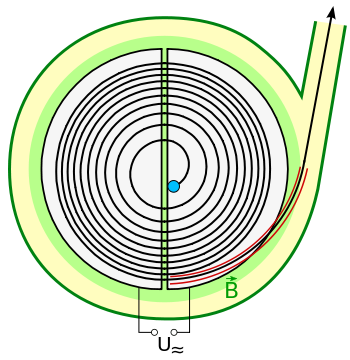
\includegraphics[width=0.35\textwidth]{Zyklotron_Prinzipskizze02.png}
%	\vspace{-13pt}
%	\caption{Prinzipskizze eines Zyklotrons}
%	\vspace{-5pt}	
%	
%\end{wrapfigure}

%\subsubsection{Anwendung}

% Some Formula:

%\begin{equation}
%	x= \frac{y \cdot 13 \pi z}
%			{\cos \alpha}
%\end{equation}

%%%%%%%%%%%%%%%%%%%%%%%
% Eigentlicher Beginn %
%%%%%%%%%%%%%%%%%%%%%%%

\section{Elektronenmasse bestimmen per Fadenstrahlrohr}

Nach einem Wien'schen Geschwindigkeitfilter werden die Elektronen in ein homogenes magnetisches Feld geleitet, das senkrecht auf der Ebene der Elektronenbahn steht. Dadurch werden alle Elektronen gemäß der Lorentz'schen Regel mit der selben Kraft auf eine Kreisbahn gezwungen.\label{Kreisbahn}

Dieser Zentripetalkraft wirkt einzig die Zentrifugalkraft entgegen. Da die Geschwindigkeiten aller Elektronen gleich sind, ist diese nur noch von der Masse der Elektronen abhängig. Diese bestimmt also den Radius der Kreisbahn und ein schwereres Teilchen träfe in der Zeichnung auf Buchseite 128 weiter oben auf.
